\documentclass[12pt,openright,oneside,a4paper,brazil]{abntex2}


\usepackage{amsmath}
\usepackage{amsmath,amsthm,amsfonts,amssymb,amscd}
\usepackage{graphicx}
\usepackage[ruled,vlined]{algorithm2e}
\graphicspath{{./imagens/}{./}} % where to search for the images

%opening
\titulo{Trabalho de Analise de Algoritmos}
\autor{Felipe Augusto Ferreira de Castro \textbf{Matrícula:} 11711BCC033\\Sarah Hanna VB  Silva \textbf{Matrícula:} 11621BCC021\\ Renata Cristina Gomes da Silva \textbf{Matrícula:} 11721BCC012}
\data{2021}
\local{Universidade Federal de Uberlândia}
\begin{document}

\imprimircapa
\newpage
\tableofcontents

\chapter{Coloração de Grafos}

\section{Pseudo-código}

O problema de coloração de grafos é um problema bastante discutido na literatura da área e possui vários algoritmos para soluciona-lo. Portanto, nesta seção apresentaremos o algoritmo usado em nosso trabalho para encontrar a disposição de cores e posteriormente discutiremos a eficiência do algoritmo. A seguir o algoritmo utilizado apresentado em pseudo-código.\\

\begin{algorithm}[H]
\SetAlgoLined
\KwIn{grafo}
\KwOut{Lista com as cores de cada vertice}
declare uma variavel flag;

faça flag = verdadeiro;

atribua a cor 0 para todos os vertices do grafo\;

inicie pelo primeiro vértice do grafo\; 

\While{não atribuido uma cor a todos os vertices}{	
	
	\While{para todos os vertices adjacentes }
	{ 
		olhe a cor do vertice adjacente\;
		
		\eIf{possui a mesma cor que o vertice adjacente}
		{
			
		 faça flag = falso\;
		 	
		 pare o laço\;		
		}{}
	}
	\eIf{flag =  verdadeiro}{
		proximo vertice;
		
	}{  
		faça flag = verdadeiro\;
	    some 1 a cor deste vertice\;
	}
}
\caption{Coloraçao de Grafos}
\end{algorithm}

Explicando de maneira mais informal o algoritmo se resume em alguns passos:
\begin{itemize}
	\item Para cada vértice $v$ do grafo $G$ vamos olhar as cores de seus vertices adjacentes;
	\item vamos avançando na lista de cores até encontrar uma cor, a qual não foi atribuída a nenhum vértice adjacente a $v$;
	\item atribuímos a cor encontrada ao vertice $v$; 
\end{itemize}

\section{Estrutura de dados}
Visto o algoritmo para coloração apresentado na seção anterior foi decidido estruturar o grafo de maneira a facilitar encontrar os vértices adjacentes de cada vértice $v$  do grafo $G$. Desta forma, cada vértice é uma estrutura que possui duas informações:
\begin{itemize}
	\item valor da cor atribuída ao vértice;
	\item uma lista de identificadores dos vértices adjacentes;
\end{itemize}

A identificação do vértice adjacente $v_d$ é feita com um indexador da posição de $v_d$ na lista de vértices do grafo $G$.

A Estrutura do grafo é constituída de duas informações: 
\begin{itemize}
	\item Lista de vértices presentes no grafo(o indexador do vértice nessa lista é o identificador do vértice);
	\item Quantidade de arestas presentes no grafo;
\end{itemize}

Utilizando-se desta estrutura, encontrar os vértices adjacentes de um vértice $v$ se resume a apenas percorrer uma lista, excluída a necessidade de verificar se o vértice $v_d$ é adjacente a $v$.

\section{Desenvolvimento do Trabalho}
O programa foi desenvolvido na linguagem Python devido a facilidade de encontrar ferramentas prontas para manipular estruturas de dados e o conhecimento prévio que os autores deste trabalho tinham sobre a linguagem. Além disso, o ambiente de desenvolvimento  usado foi o Visual Studio Code.


\subsection{Grafos}   
Quantos aos grafos, foram utilizados 5 grafos, no formato DIMACS, os quais serão apresentados a seguir. 

\begin{enumerate}
	\item 	\textbf{Grafo 1} \newline
		vertices: 10 , arestas: 15, \newline
		a 0 1, \newline
		a 0 2, \newline
		a 0 3, \newline
		a 1 4, \newline
		a 1 8, \newline
		a 2 6, \newline
		a 2 7, \newline
		a 3 5, \newline
		a 3 9, \newline
		a 4 5, \newline
		a 4 7, \newline
		a 5 6, \newline
		a 6 8, \newline
		a 7 9, \newline
		a 8 9;
		
		\includegraphics[width=5cm]{grafo1.png}

		
		Fonte: O enunciado deste trabalho
	\item \textbf{Grafo 2} \newline 
		vertices: 9, arestas: 14, \newline
		a 0 3, \newline
		a 0 1, \newline
		a 1 2, \newline
		a 1 3, \newline
		a 2 4, \newline
		a 3 4, \newline
		a 3 6, \newline
		a 3 7, \newline
		a 4 5, \newline
		a 4 7, \newline
		a 4 8, \newline
		a 5 8, \newline
		a 6 7, \newline
		a 7 8;
		
		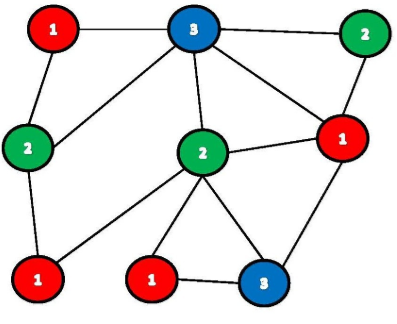
\includegraphics[width=5cm]{grafo2.png}
		
		Fonte: \url{https://coloringbee.blogspot.com/2018/09/coloring-graph-example.html}
	\item \textbf{Grafo 3} \newline
		vertices: 8, arestas: 12, \newline
		a 0 5, \newline
		a 0 6, \newline
		a 0 7, \newline
		a 1 4, \newline
		a 1 6, \newline
		a 1 7, \newline
		a 2 4, \newline
		a 2 5, \newline
		a 2 7, \newline
		a 3 4, \newline
		a 3 5, \newline
		a 3 6;
		
		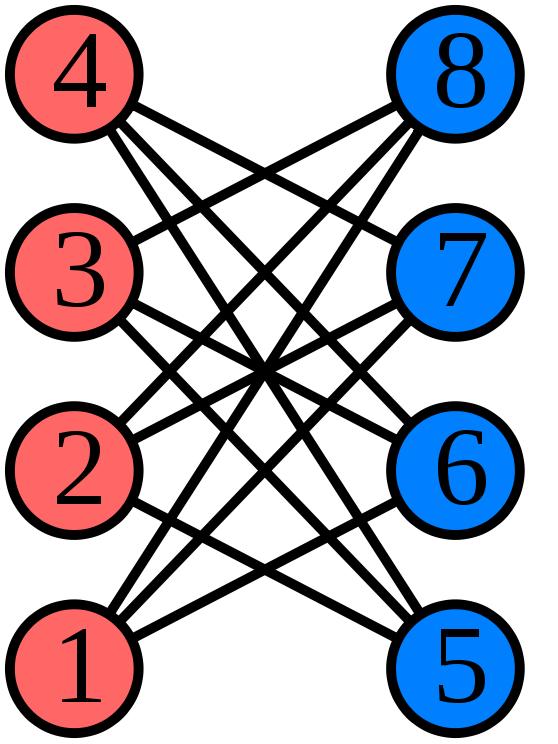
\includegraphics[width=4cm,height=5cm]{grafo3.png}
		
		Fonte: \url{https://handwiki.org/wiki/Grundy_number}
	\item \textbf{Grafo 4}\newline
		vertices: 11, arestas: 13
		a 0 1, \newline
		a 0 2, \newline
		a 1 2, \newline
		a 1 3, \newline
		a 2 3, \newline
		a 2 6, \newline
		a 3 5, \newline
		a 4 5, \newline
		a 6 7, \newline
		a 6 9, \newline
		a 7 8, \newline
		a 7 9, \newline
		a 9 10;
		
		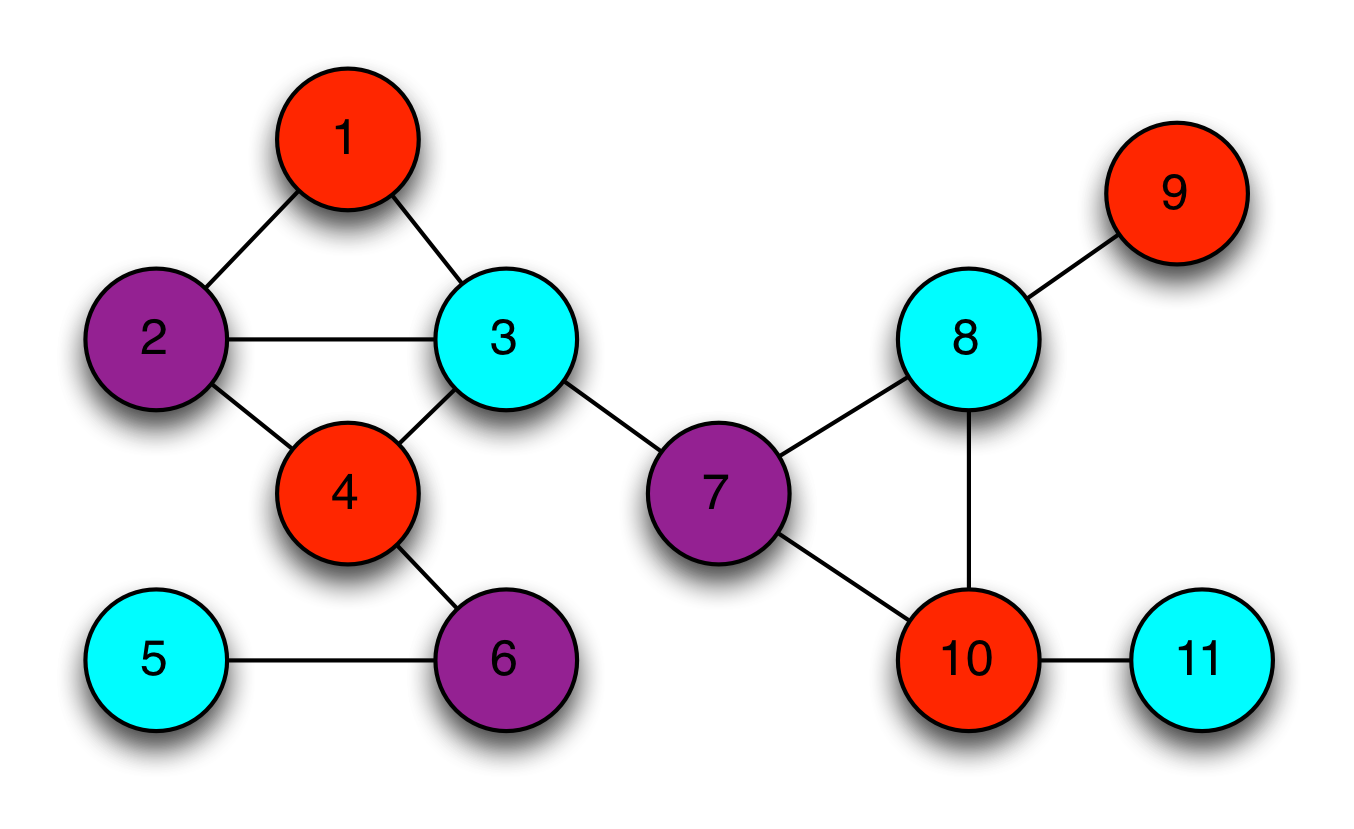
\includegraphics[width=5cm]{grafo4.png}
		
		Fonte: \url{https://blog.cryptographyengineering.com/2014/11/27/zero-knowledge-proofs-illustrated-primer/}
	\item \textbf{Grafo 5}\newline
		vértices: 7393, arestas: 25569. \newline
	Devido a quantidade de vértices e arestas não é viável apresentar aqui a estrutura do grafo. Visto isso, vamos disponibiliza-lo no seguinte link: \url{https://github.com/felipe-2705/Trabalho-AA/blob/master/grafos/grafo5.dimacs}
	
	Fonte: \url{https://lcs.ios.ac.cn/~caisw/graphs.html}
\end{enumerate}

\subsection{Execução}
Aqui mostraremos o resulta das colorações para os grafos de 1 a 4 e compararemos com os resultados já conhecidos para cada um dos casos. Além de mostrar o tempo de execução para 100 execuções para cada grafo e suas medias. As bibliotecas utilizada para tal foram \textit{statistics} e \textit{Matplotlib} 
\begin{enumerate}
	\item \textbf{Grafo 1}
	
		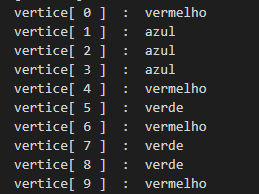
\includegraphics[width=4cm,height=4cm]{Coloracao-grafo1.png}
		\includegraphics[width=5cm]{grafo1.png}
		
		Podemos observar que para este grafo o algoritmo atingiu uma solução ótima, utilizando 3 cores para colorir o grafo 1;
		Os tempos de execução são mostrados a seguir:
		
		\begin{center}
			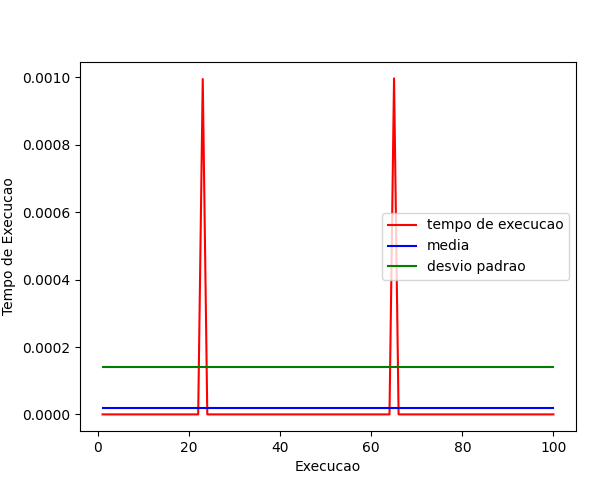
\includegraphics[width=8cm,height=8cm]{grafico-grafo1.png}
			
		\end{center}
	\item \textbf{Grafo 2}
	
	    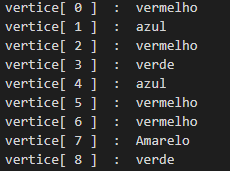
\includegraphics[width=4cm,height=4cm]{Coloracao-grafo2.png}
	    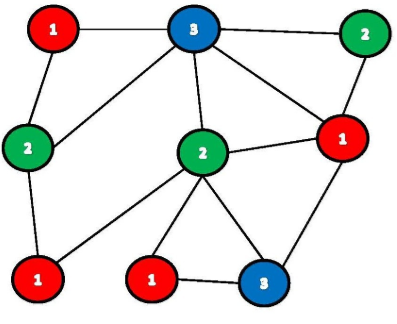
\includegraphics[width=5cm]{grafo2.png}
	    
	    Para este grafo a coloração atingida pelo algoritmo não foi a solução ótima, utilizando 4 cores para colorir o grafo, sendo o ideal 5 cores;
	   Os tempos de execução são mostrados a seguir:
	    
	    \begin{center}
	    	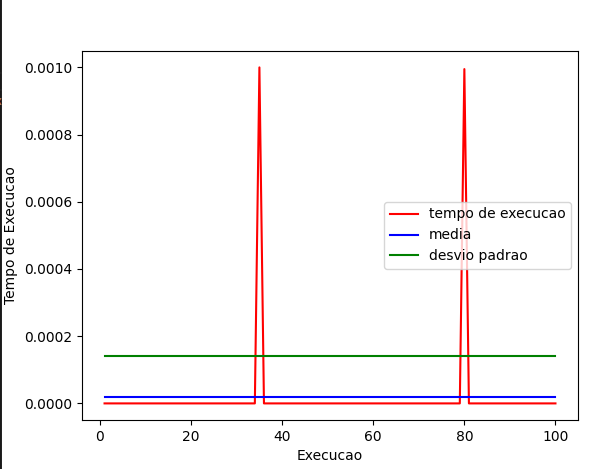
\includegraphics[width=8cm,height=8cm]{grafico-grafo2.png}
	    	
	    \end{center}
	    
	\item \textbf{Grafo 3}
		
		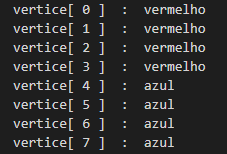
\includegraphics[width=4cm,height=4cm]{Coloracao-grafo3.png}
		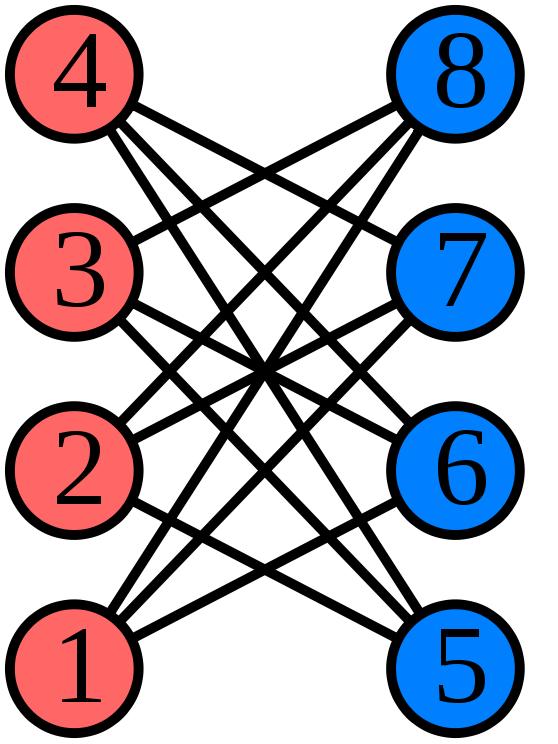
\includegraphics[width=4cm,height=5cm]{grafo3.png}
		
		Para o Grafo bipartido a solução ótima foi atingida de 2 cores;
		Os tempos de execução são mostrados a seguir:
		
		\begin{center}
			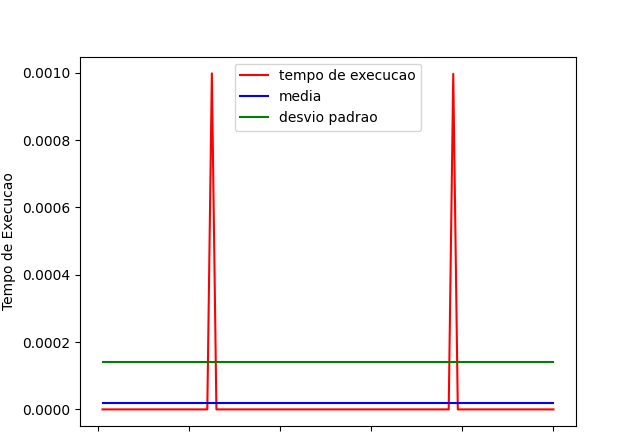
\includegraphics[width=8cm,height=8cm]{grafico-grafo3.png}
			
		\end{center}
	
	\item \textbf{Grafo 4}
	
	 	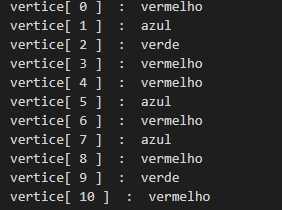
\includegraphics[width=4cm,height=4cm]{Coloracao-grafo4.png}
	 	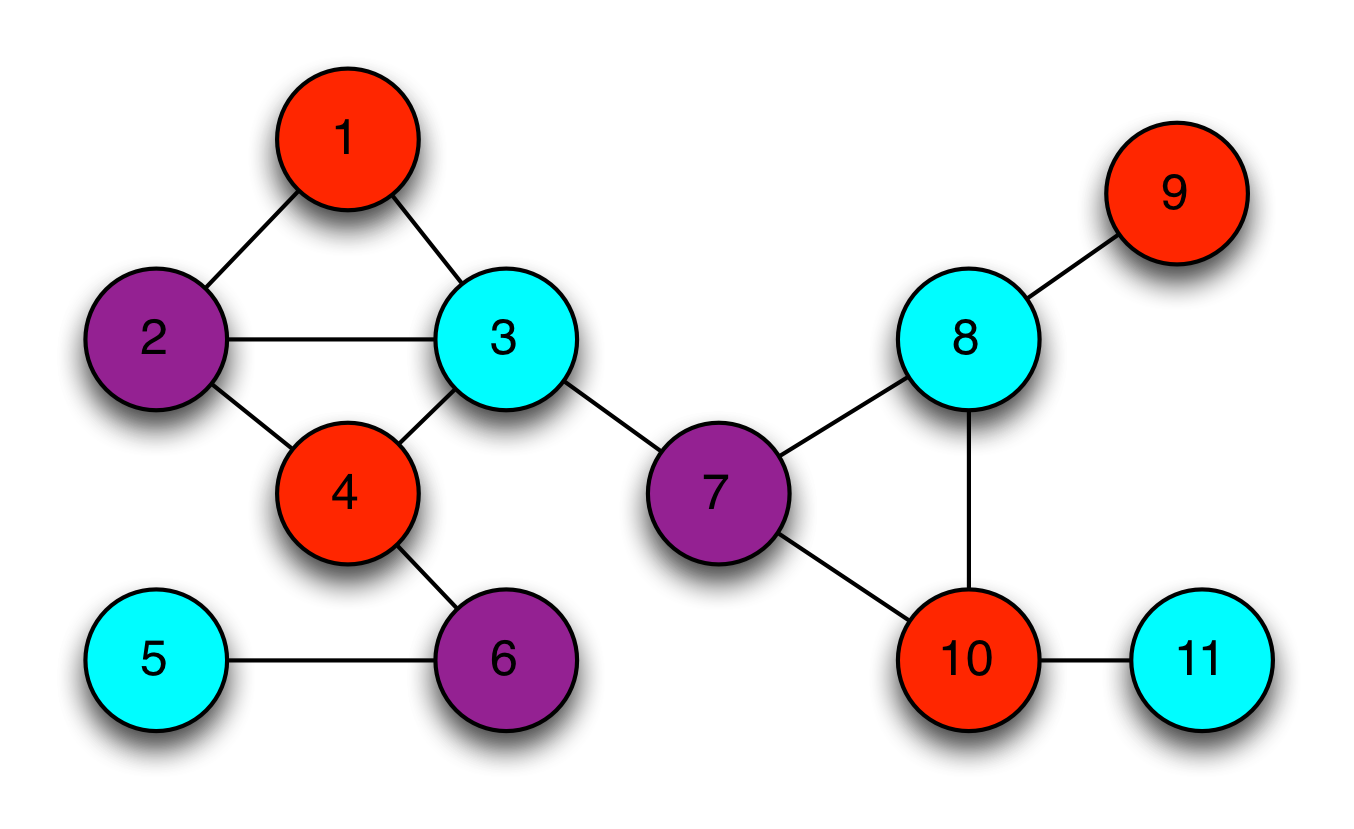
\includegraphics[width=5cm]{grafo4.png}
		 
		Para este caso também foi obtido um resultado ótimo de 3 cores para a coloração do grafo;
		Os tempos de execução são mostrados a seguir:
		
			\begin{center}
			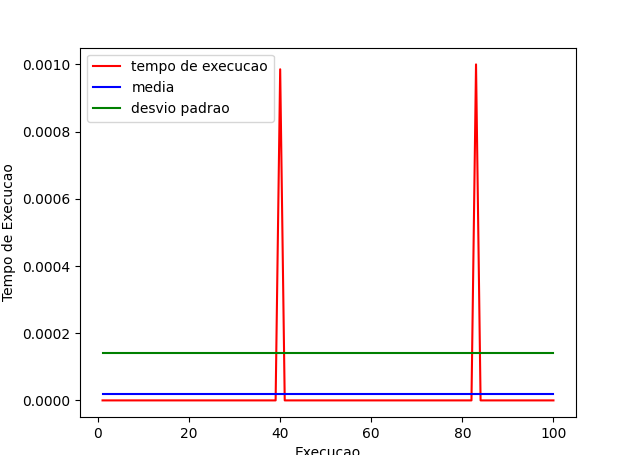
\includegraphics[width=8cm,height=8cm]{grafico-grafo4.png}
			
		\end{center}
		
	\item \textbf{Grafo 5}
	
		Devido ao tamanho do grafo 5 não será apresentada uma comparação das coloração realizada, porém foram utilizada 3 cores. Não se sabe se este é a coloração ótima;
		Para os tempos de execução foi obtido um desvio padrão de $0.004048385768314759$. Para o caso apresentado abaixo o desvio padrão não foi incluído e os seguintes tempos foram obtidos: 
		
		\begin{center}
			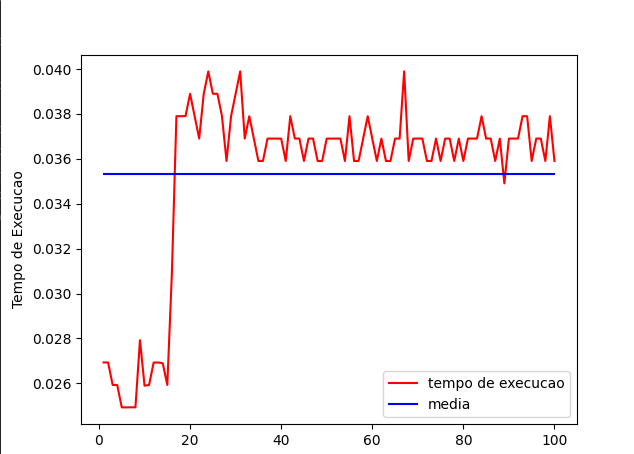
\includegraphics[width=8cm,height=8cm]{grafico-grafo5.png}
			
		\end{center}
		
\end{enumerate}
\section{conclusão}
A seção anterior apresentou os resultados para os cinco gráficos descritos neste trabalho. Nesta seção iremos discutir estes resultados. Podemos observar que o algoritmo conseguiu atingir para os grafos 1,3,4 uma solução ótima e para o grafo 2 uma  bastante próximo do ótimo, visto que utilizou apenas uma cor a mais, o que é um bom resultado para o algoritmo. 
Quanto aos tempos de execução podemos ver que para os grafo 1 ao 4 permanece bastante próximo de 0 segundos, tendo pouquíssima variação como podemos observar pelo valor do desvio padrão. Por isso foi adicionado o grafo 5, cujo numero de vértices e arestas é bastante superior ao aos demais. O grafo 5 manteve tempo de execução entre 0.035 e 0.040 para as 100 execuções e um desvio padrão baixo, o que é um aumento abaixo do esperado, visto a diferença de grandeza entre o grafo 5 e os demais.

\section{Vídeo}
O vídeo apresentando uma execuçao desse trabalho encontra-se em : \url{https://web.microsoftstream.com/video/05dafa84-e1f3-44f9-b7fe-269058867a08}

\chapter{Caixeiro Viajante} 

Este algoritmo foi desenvolvido em python e pode ser encontrado em \url{https://github.com/felipe-2705/Trabalho-AA/tree/master/caixeiro}. Tanto os códigos quanto o grafo se encontram nesse link. 
Sobre o grafo, não será apresentado aqui por ser muito extenso constituído de 38 vértices e 1444 arestas. Porém pode ser acessado no link citado anteriormente. Este grafo é dividido em um arquivo de distancias ("distancia.txt") e um com os dados dos vértices ("cidades.txt").  

\section{Resultados}
O algoritmo percorreu caminhos com 38 entradas obtendo os seguintes resultados: 
      \begin{enumerate}
      	\item Execução:	\\
			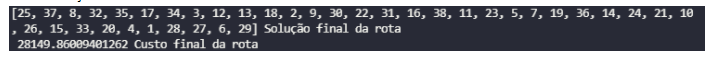
\includegraphics[scale=0.8]{caixeiro-execução1.png}
      	\item Execução:\\
			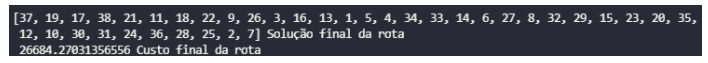
\includegraphics[scale=0.8]{caixeiro-execução2.png}		
      	\item Execução:\\
			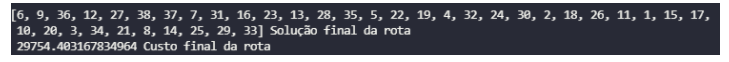
\includegraphics[scale=0.8]{caixeiro-execução3.png}		
      	\item Execução:\\
			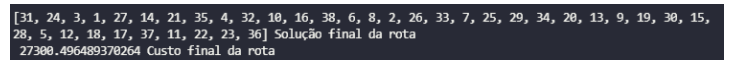
\includegraphics[scale=0.8]{caixeiro-execução4.png}
      	\item Execução:\\
			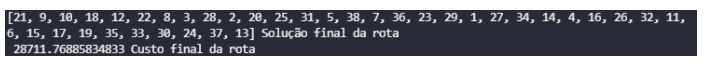
\includegraphics[scale=0.8]{caixeiro-execução6.png}		    	
      \end{enumerate}
A seguir apresentamos o gráficos dos resultados, no eixo y temos cada grafo sendo correspondente a uma execução e no eixo x o tempo de execução, em segundos, gasto para concluir o algoritmo.\\
		      	\includegraphics[scale=0.8]{execução.png}		\\
Ao final dos testes foi obtido um tempo médio de 28119 segundos com um desvio padrão de 1199 segundos. 
\end{document}
